\documentclass{article}
\usepackage[T1]{fontenc}
\usepackage{lmodern}
\usepackage{graphicx}
\usepackage{amsmath,amssymb}
\usepackage[a4paper,margin=2cm]{geometry}
\usepackage[absolute,overlay]{textpos}
\setlength{\TPHorizModule}{1mm}
\setlength{\TPVertModule}{1mm}
\usepackage[indonesian]{babel}
\usepackage{hyperref}
\setlength{\emergencystretch}{2em}
% unit: Halaman 20

\begin{document}

% === Halaman 20 (llm) ===

\vspace{231.66mm}

\begin{itemize}
    \item $E$ adalah fungsi ekspansi yang memperluas blok $R_{i-1}$ 32-bit menjadi blok 48 bit.
    \item Fungsi ekspansi direalisasikan dengan matriks permutasi ekspansi:
\end{itemize}

\begin{tabular}{|c|c|c|c|c|c|c|c|c|c|c|c|c|c|c|c|}
\hline
32 & 1 & 2 & 3 & 4 & 5 & 4 & 5 & 6 & 7 & 8 & 9 \\
\hline
8 & 9 & 10 & 11 & 12 & 13 & 12 & 13 & 14 & 15 & 16 & 17 \\
\hline
16 & 17 & 18 & 19 & 20 & 21 & 20 & 21 & 22 & 23 & 24 & 25 \\
\hline
24 & 25 & 26 & 27 & 28 & 29 & 28 & 29 & 30 & 31 & 32 & 1 \\
\hline
\end{tabular}

\vspace{20mm}

% deskripsi: Diagram alur proses enkripsi yang melibatkan fungsi ekspansi E, operasi XOR dengan kunci Ki, matriks substitusi S-box, dan permutasi P(B).
% bbox normalisasi: [0.6300, 0.1000, 0.9900, 0.8800]
\begin{textblock*}{75.60mm}(132.30mm,29.70mm)
\noindent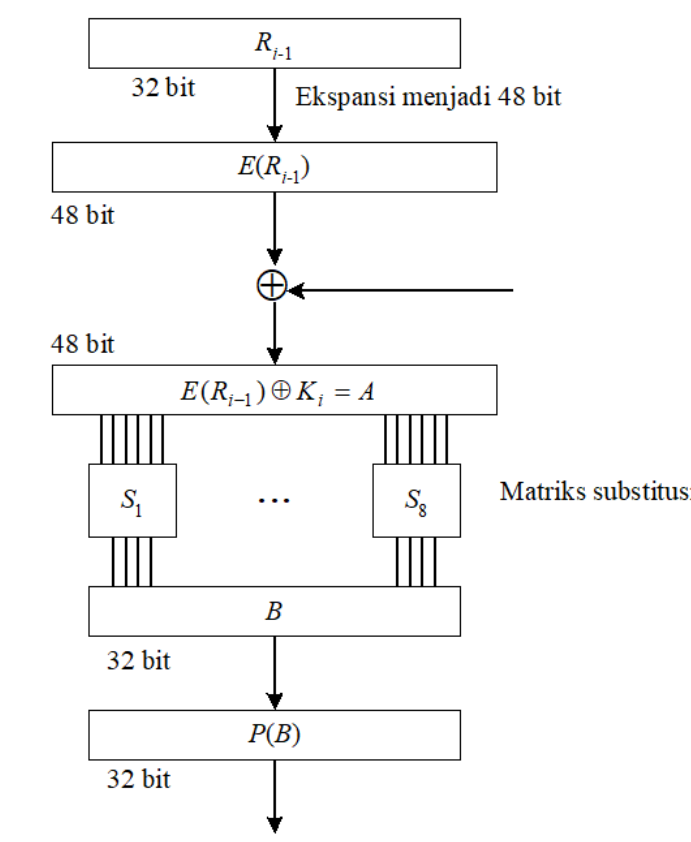
\includegraphics[width=75.60mm,height=231.66mm]{../../images/llm/page_020_img_01.png}%
\end{textblock*}

\end{document}
